\documentclass{standalone}
\usepackage{libertine}
\usepackage[dvipsnames]{xcolor}
\usepackage{tikz}
\usepackage{fix-cm}
\setlength{\parskip}{0pt}
\setlength{\baselineskip}{0pt}
%\usetikzlibrary{fit}
\usetikzlibrary{calc}
\usetikzlibrary{decorations.markings}
\usetikzlibrary{decorations.shapes}
\usetikzlibrary{decorations.pathreplacing}
\usetikzlibrary{intersections}
\usetikzlibrary{patterns}
\tikzset{%
  from end of path/.style={
    insert path={
      \pgfextra{%
        \expandafter\pgfprocesspathextractpoints%
          \csname tikz@intersect@path@name@#1\endcsname%
        \pgfpointlastonpath%
        \pgfgetlastxy\lastx\lasty
      }
      (\lastx,\lasty)
}}}
\tikzset{-dot-/.style={decoration={
  markings,
  mark=at position #1 with {\fill[color=red] circle (0.5mm);}},postaction={decorate}}}  
\tikzset{-dot3-/.style={decoration={
  markings,
  mark=at position #1 with {\draw[-,draw=none,fill=white](0.025,-0.05) -- (-0.025,0.05) -- (-0.015,0.05) -- (0.035,-0.05) -- cycle;%
\draw[-,color=black](0.025,-0.05) -- (-0.025,0.05); \draw[-,color=black](0.035,-0.05) -- (-0.015,0.05);}},postaction={decorate}}}
    \tikzset{
        hatch distance/.store in=\hatchdistance,
        hatch distance=10pt,
        hatch thickness/.store in=\hatchthickness,
        hatch thickness=2pt
    }
\begin{document}
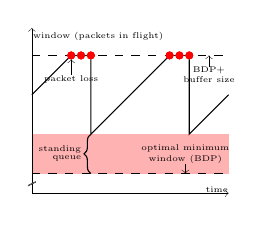
\begin{tikzpicture}
    
    \makeatletter
    \pgfdeclarepatternformonly[\hatchdistance,\hatchthickness]{flexible hatch}
    {\pgfqpoint{0pt}{0pt}}
    {\pgfqpoint{\hatchdistance}{\hatchdistance}}
    {\pgfpoint{\hatchdistance-1pt}{\hatchdistance-1pt}}%
    {
        \pgfsetcolor{\tikz@pattern@color}
        \pgfsetlinewidth{\hatchthickness}
        \pgfpathmoveto{\pgfqpoint{0pt}{0pt}}
        \pgfpathlineto{\pgfqpoint{\hatchdistance}{\hatchdistance}}
        \pgfusepath{stroke}
    }
    \makeatother
 
\draw[dashed] (0,1) -- ++(2.5,0);
\node[align=center,font=\fontsize{3pt}{0}\selectfont,inner sep=0mm] at (2.25, 0.75) (bufferSizeLabel) {BDP+\\ buffer size};
\draw[->, line width=0.05mm] (bufferSizeLabel) -- (2.25,1);
\draw[name path=A] (0,0.5)-- ++(0.5, 0.5);
\draw[from end of path=A, name path=B, -dot-=0, -dot-=0.5, -dot-=1] -- ++(0.25,0);
\node[align=center,font=\fontsize{3pt}{0}\selectfont,inner sep=0mm] at (0.5, 0.7) (lossLabel) {packet loss};
\draw[->, line width=0.05mm] (lossLabel) -- (0.5,0.95);
\draw[from end of path=B, name path=C] ++(0,-0.5mm) -- ++(0,-0.95cm) -- ++(1,1);
\draw[from end of path=C, name path=D, -dot-=0, -dot-=0.5, -dot-=1] -- ++(0.25,0);
\draw[from end of path=D, name path=E] ++(0,-0.5mm) -- ++(0,-0.95cm) -- ++(0.5,0.5);

%\fill[pattern=flexible hatch, pattern color=red, hatch distance=1mm, hatch thickness=0.01mm] (0,0) rectangle ++(2.5,-0.5);
\draw[draw opacity=0,fill=red,fill opacity=0.3] (0,0) rectangle ++(2.5,-0.5);
%\draw[name path=A] (0,-0.5)-- ++(2.5, 0);

\draw[draw,decorate,decoration={brace,mirror}] (0.75,0) -- (0.75,-0.5) node [midway,left,align=right,font=\fontsize{3pt}{0}\selectfont] {standing\\ queue};

\draw[dashed] (0,-0.5) -- ++(2.5,0);
\node[align=center,font=\fontsize{3pt}{0}\selectfont,inner sep=0mm] at (1.95,-0.25) (optimal) {optimal minimum\\ window (BDP)};
\draw[->, line width=0.05mm] (optimal) -- ++(0,-0.25);

\draw[->, line width=0.05mm] (0,-0.75) -- ++(2.5,0);
\node[align=center,font=\fontsize{3pt}{0}\selectfont,inner sep=0mm] at (2.35, -0.7) (time) {time};
\draw[draw=none, line width=0.05mm] (0,-0.8) -- ++(2.5,0);

\draw[->, line width=0.05mm, -dot3-=0.055] (0,-0.75) -- ++(0,2.1);
\node[anchor=north west, align=center,font=\fontsize{3pt}{0}\selectfont,inner sep=0mm] at (0.01, 1.3) (window) {window (packets in flight)};
\draw[draw=none, line width=0.05mm] (-0.05,-0.75) -- ++(0,2.1);

%\draw[draw,decorate,decoration={brace,mirror}] (0.75,0) -- (1.75,0) node [inner sep=0, outer sep=0,midway,below,yshift=-1.25mm,font=\fontsize{3pt}{0}\selectfont] {interval};
%\draw[densely dotted] (1.75,0) -- (1.75,0.95);
\end{tikzpicture}
\end{document}
